\chapter{Simulation Environment}
The discussion of the flight mechanics in Chapter 2 and the equations of motion presented in Chapter 4 would be meaningless if the flight vehicle is not being controlled to a final destination. Up until this point, this thesis has covered the navigation architecture in the overarching Guidance, Navigation, and Control (GNC) flight vehicle model. This chapter will expand on both the guidance and control architecture utilized for this work. Although these are not the primary focus of this thesis, they are important to discuss if others wish to replicate the study.

\section{Guidance System}
The guidance system for a flight vehicle holds responsibility for providing reference points to the controllers that process them into actuation of the control surfaces and engine controls. These reference points are calculated on a number of variables including the atmospheric conditions, estimated pose of the aircraft, and engine efficiency. For the purposes of this work, the primary goal of the guidance system is to accept a user-defined trajectory consisting of waypoints defined in the local navigation frame and convert these into aircraft heading, pitch, throttle, and propeller pitch reference commands for the controllers to interpret. The following subsection provides an overview of creating trajectories for the guidance system.

\subsection{Waypoint Generation}
In this work, generation of waypoints is a simple process where the user manually picks a trajectory using Google Earth~\cite{GoogleEarth}. Once a trajectory is created (Figure~\ref{fig:googleEarth}) and saved as a \textit{kml} file, it can be brought into MATLAB and converted into a matrix of values in the local navigation frame. Note, at this point, it may be beneficial to alter the altitude values such that the aircraft climbs, descends, or maintains a certain altitude during the length of the simulation. The conversion of the \textit{kml} file can be done using the \textit{KML Toolbox} from~\cite{KMLToolboxFile}.

\begin{figure}[!ht]
    \centering
    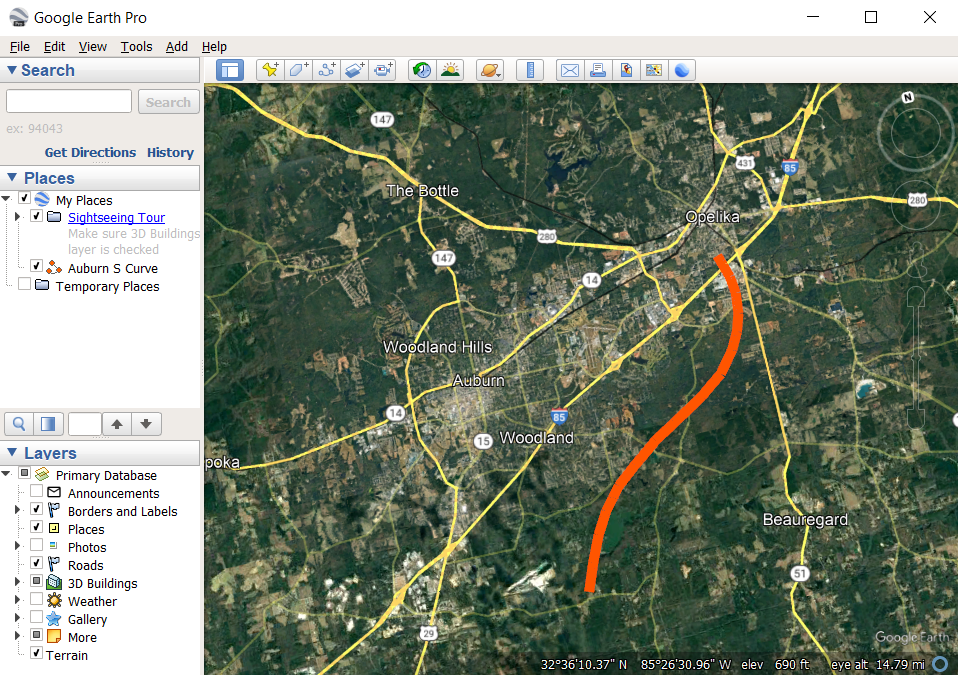
\includegraphics[width=0.75\linewidth]{Figures/auburnScurve.png}
    \caption{A custom trajectory created in Google Earth for the guidance system discussed in this work.}\label{fig:googleEarth}
\end{figure}

Once the trajectory is imported into the model, it is used within the guidance system to produce reference commands of desired heading, pitch, throttle, and propeller pitch. This work uses the \textit{uavWaypointFollower} class provided by the UAV Toolbox in MATLAB\@. Other methods of waypoint following can be used, as long as they output the aforementioned reference commands.

The waypoint follower calculates the reference heading and pitch by using trigonometric relationships between the flight vehicles current pose and the selected waypoints position. The throttle is chosen such that time between waypoints is consistent. The propeller pitch is calculated such that propeller efficiency is maximized. The calculation of propeller efficiency was discussed in Chapter 2. These reference commands are passed to the control scheme to map controlling values to normalized aircraft stick movements, throttle lever position, and propeller lever position. This processed in discussed in the next section.

\section{Control Scheme}

As stated previously, the guidance system and control law are not the primary focus of this work. Because of this, only classical Proportional-Integral-Derivative (PID) controllers are used to actuate the controls surfaces to the desired values from the guidance system. During the simulations presented during the results of this thesis, only four of the available eleven inputs are being controlled to maintain the desired trajectory of the aircraft. Table~\ref{tbl:controls} lays out the available inputs available for the Diamond-DA40 modeled in this work.

\begin{table}[!ht]
    \caption{List of available, controllable inputs to the Diamond DA40 modeled in this thesis.}\label{tbl:controls}
    \centering
    \begin{tabular}{llc}
        \toprule
        \textbf{Input}     & \textbf{Definition}                                               & \textbf{Controlled} \\
        \midrule
        Lateral Stick      & L/R movement of pilot stick, maps to \(\delta_a\)                 & \(X\)               \\
        Longitudinal Stick & Fwd/Aft movement of pilot stick, maps to \(\delta_e\)             & \(X\)               \\
        Rudder Pedals      & In/Out position of left/right rudder pedals, maps to \(\delta_r\) &                     \\
        Throttle Lever     & Lever \% w.r.t.\ throttle, maps to engine RPM          & \(X\)               \\
        Propeller Lever    & Lever \% w.r.t.\ propeller pitch angled normal to freestream      & \(X\)               \\
        Mixture Lever      & Lever \% w.r.t.\ fuel-to-air ratio within engine                  &                     \\
        Left Brake         & Position of L rudder pedal when a/c is on ground                  &                     \\
        Right Brake        & Position of R rudder pedal when a/c is on ground                  &                     \\
        Aileron Trim       & \(\delta_a\) needed to maintain a/c stability                     &                     \\
        Rudder Trim        & \(\delta_r\) needed to maintain a/c stability                     &                     \\
        Elevator Trim      & \(\delta_e\) needed to maintain a/c stability                     &                     \\
        \bottomrule
    \end{tabular}
\end{table}

Control of the lateral stick is a function of two open-loop controllers based on the commanded heading from the guidance system and the current heading and roll angle of the aircraft. It is assumed that the nose of the aircraft always points in the direction of the aircraft's velocity for the purpose of this thesis. Figure~\ref{fig:latstickcontrol} shows the two open-loop controllers working in series with their listed gains for more detail.

\begin{figure}[!ht]
    \centering
    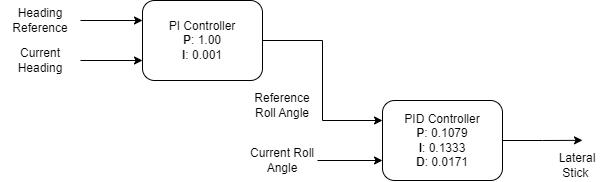
\includegraphics[width=0.75\linewidth]{Figures/latstickcontrol.drawio.png}
    \caption{Block diagram of lateral stick control through two open-loop, PID controllers.}\label{fig:latstickcontrol}
\end{figure}

The movement of the pilot stick in the longitudinal direction is a function of the commanded altitude from the guidance systems and the current altitude and pitch of the aircraft. Two open-loop PID controllers are used in series to control the pilot stick that actuates the elevator to the correct deflection angle. Figure~\ref{fig:longstickcontrol} shows a block diagram of the two controllers with their proportional, integral, and derivate gains.

\begin{figure}[!ht]
    \centering
    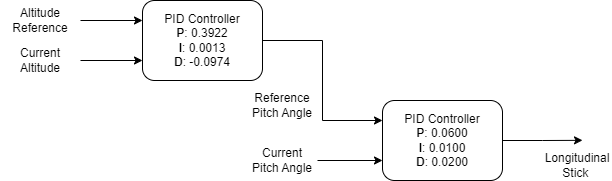
\includegraphics[width=0.75\linewidth]{Figures/longstickcontrol.drawio.png}
    \caption{Block diagram of longitudinal stick control through two open-loop, PID controllers.}\label{fig:longstickcontrol}
\end{figure}

The throttle and propeller lever controllers use a PID and PI controller to correct their inputs. Table~\ref{tbl:throttleProp} displays their controller gains. The throttle control is based on the commanded and current airspeed of the aircraft where the propeller lever is controlled based on maintaining at least \(90\% \) propeller efficiency. The airspeed for the throttle control is defined as the magnitude of the aircraft's velocity.

\begin{table}[!ht]
    \caption{Gains for the throttle and propeller lever open-loop PID controllers.}\label{tbl:throttleProp}
    \centering
    \begin{tabular}{cccc}
        \toprule
        Controller      & Proportional & Integral  & Derivative \\
        \midrule
        Throttle Lever  & \(0.498\)    & \(0.098\) & \(-0.184\) \\
        Propeller Lever & \(0\)        & \(1\)     & \(0\)      \\
        \bottomrule
    \end{tabular}
\end{table}

The controllers provide inputs such that actuation of the control surfaces are deflected properly and can guide the aircraft in the desired direction at the desired speed while maintaining propeller efficiency. With the implementation of the guidance system and control law, the full GNC loop is now complete. The following section describes the disturbances modeled on the aircraft so that controller inputs and outputs are different when running Monte-Carlo simulations for further analysis of the proposed navigation filter architecture.

\section{Disturbance Modeling}

As specified in Equation~\ref{eq:eulerIntegration}, the dynamics of the aircraft are disturbed by external forces that changes the behavior of the aircraft between simulations of the same trajectory. Ultimately, these changes lead to different control inputs and allow the Monte-Carlo analyses to emphasize the affect of the proposed FVDM navigation filter.

For the study presented in this thesis, two disturbances are modeled {--} a wind model and uncertainties in the current altitude. The wind model is represented as a zero-mean white noise process from~\cite{khaghaniAutonomousVehicleDynamic2016}. Changes in the wind are important to simulation as wind greatly affect aircraft trajectories in the real-world. The modeling of wind as a white noise process provides a stochastic process that more closely resembles wind data collected from actual data collections~\cite{mwenegohaModelbasedTightlyCoupled2020}. In Chapter 2, it is clear that the pressure, temperature and density calculation stem from the ISA model; however, aircraft do not use this model on board. To simulate changes in these atmospheric parameters, measurements from a Pitot tube and temperature sensor are modeled as a zero-mean white noise process from~\cite{pieniazekDynamicResponsePitot2023}. Similar to the white-noise wind model, the measurements of pressure, temperature, and density must be variant enough to have different control inputs over the course of many Monte-Carlo simulations. The variance in these white noise models can be substituted for their respective variables in \(\mathbf{Q}_d\) (Equation~\ref{eq:Qd}).

\section{Conclusions}

The guidance systems and control laws provide the aircraft with meaningful control surface deflection that guide the aircraft to the desired destination. This chapter provided an overview about how the guidance systems generates commanded control inputs from a user-defined trajectory created using Google Earth. Following the guidance system, the control law used in this thesis was covered with discussions about the PID control gains used for each of the four piloted control inputs during simulation. Finally, a discussion of the disturbances on the aircraft dynamics that influence different control inputs between simulations was described. The focus of this work is not on the guidance or controls of the flight vehicle presented in this thesis, for better detail of each the sections discussed during this chapter, the reader is asked to follow-up with the references cited above for more information.